% \chapter{CHAPITRE 4 : SAYNOTE – VISUAL IDENTITY}

% --- Introduction non numérotée ---
\begin{center}
\textbf{\large Introduction du Chapitre}
\end{center}

\noindent
Ce chapitre présente la démarche de création et les choix fondamentaux de l'identité visuelle pour VoiceNotion. Il met en avant l'importance du branding, des couleurs, de la typographie et des supports graphiques pour garantir une expérience utilisateur cohérente et mémorable, tout en valorisant la marque sur tous les supports.

\section{Introduction}
Dans ce chapitre nous parlerons de notre identité visuelle. (Couleurs, typographie, charte graphique, design commercial, ...).

\section{Logo}
\subsection{Name selection}
\begin{tcolorbox}[colback=voicenotionLightGray!10!white, title=Origine du nom]
Le nom \textbf{Saynote} a été soigneusement choisi pour refléter la mission principale de l'application : permettre aux utilisateurs de capturer instantanément leurs idées à l’aide de leur voix. Simple, intuitif et signifiant, « Saynote » incarne l’intersection entre la parole et la productivité. C’est plus qu’un nom, c’est une expérience en un mot.
\end{tcolorbox}

\textbf{Décomposition du nom~:} \textit{Saynote = Say + Note}
\begin{itemize}
    \item \textbf{Say}~: Interaction vocale, rapidité, facilité, communication naturelle.
    \item \textbf{Note}~: Capture structurée d’idées, rappels, tâches.
\end{itemize}

\noindent
Ensemble, Saynote devient une commande, un comportement et une marque : il suffit de «~dire sa note~».

\textbf{Message et sens~:}
\begin{itemize}
    \item Vous n’avez plus besoin de taper. Il suffit de parler : votre voix devient une note.
    \item Un seul geste, un seul outil, un seul résultat. Dites-le, sauvegardez-le : terminé.
\end{itemize}

\subsection{Logo selection}
Le logo VoiceNotion combine une onde vocale stylisée et la forme d’un bloc-notes, symbolisant la fusion entre la saisie vocale et l’organisation des idées. Le dégradé bleu doux évoque le calme et la clarté, tandis que les coins arrondis et le détail du coin replié ajoutent une touche conviviale et moderne.

\begin{itemize}
    \item \textbf{Simplicité} : Formes minimales, reconnaissance immédiate.
    \item \textbf{Clarté} : Chaque élément a un but précis : outil de prise de notes avec intégration vocale.
    \item \textbf{Esthétique propre} : Courbes douces, contours nets, adaptable sur fond clair ou sombre.
    \item \textbf{Symbolisme} : Rapidité, simplicité, innovation, focus.
    \item \textbf{Adaptabilité} : Le logo reste lisible et impactant à toutes tailles.
\end{itemize}

\subsection{Design methodology}
% Explication brève avant chaque figure
\noindent
\textit{La figure suivante illustre un élément clé de l'identité visuelle ou de la communication de la marque.}
\begin{figure}[H]
    \centering
    
\includegraphics[width=0.25\textwidth]{docs/visual-indentity/pictures/logo.png}
    \caption{Logo principal VoiceNotion. \newline\textit{Ce logo fusionne la notion de voix et de prise de notes, représentant la mission centrale de l'application.}}
\end{figure}

% Explication brève avant chaque figure
\noindent
\textit{La figure suivante illustre un élément clé de l'identité visuelle ou de la communication de la marque.}
\begin{figure}[H]
    \centering
    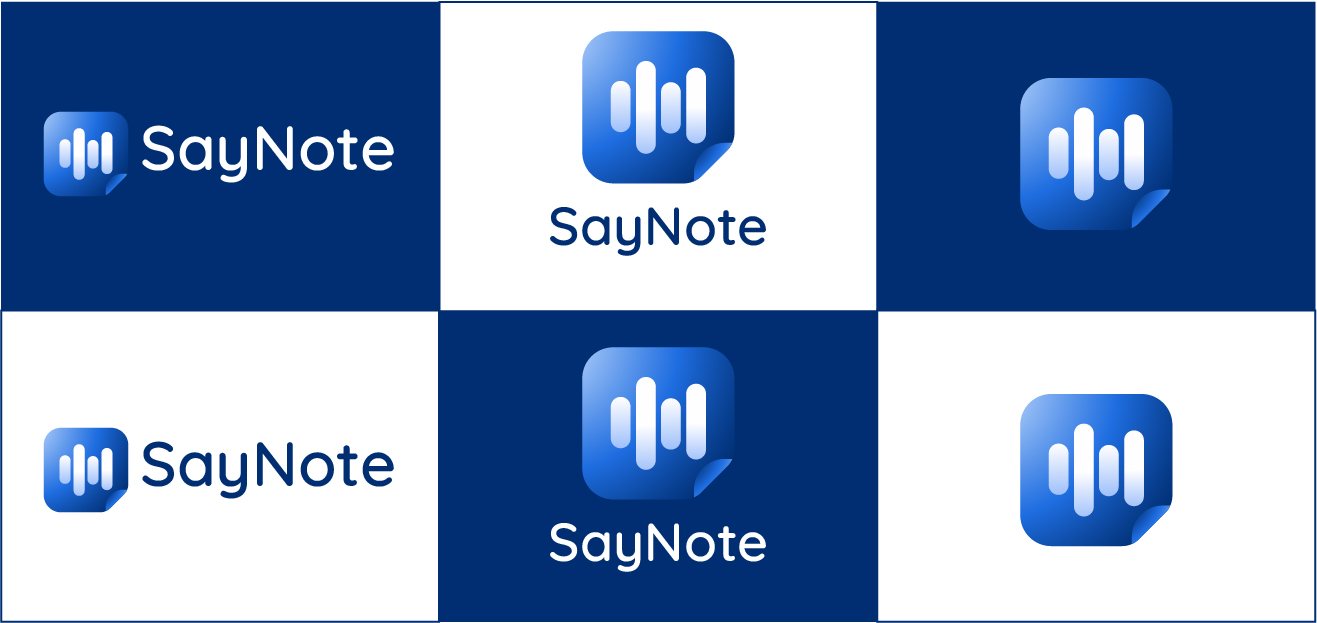
\includegraphics[width=0.7\textwidth]{docs/visual-indentity/pictures/logo-varaition-blue.jpg}
    \caption{Variante bleu du logo. \newline\textit{Cette version met en avant la modernité et la fraîcheur de la marque.}}
\end{figure}

% Explication brève avant chaque figure
\noindent
\textit{La figure suivante illustre un élément clé de l'identité visuelle ou de la communication de la marque.}
\begin{figure}[H]
    \centering
    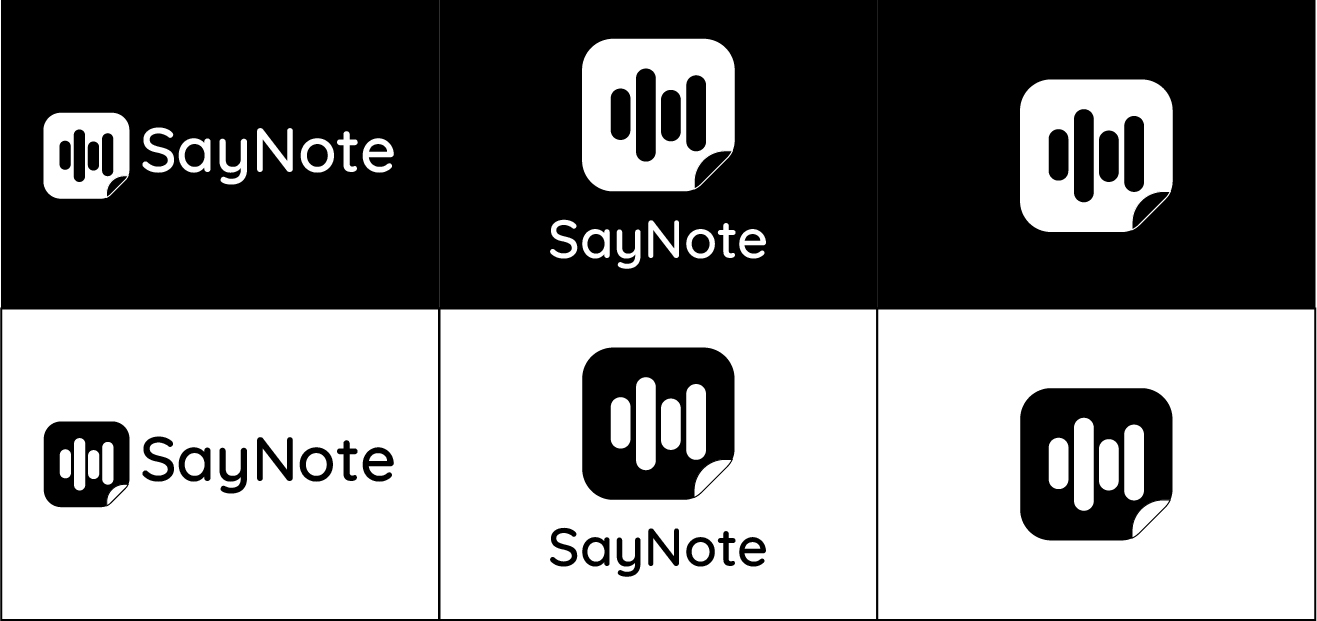
\includegraphics[width=0.7\textwidth]{docs/visual-indentity/pictures/logo-variation-black-and-white.jpg}
    \caption{Logo noir et blanc. \newline\textit{Cette variante assure la lisibilité et l'adaptabilité sur différents supports.}}
\end{figure}

\section{Typographie}
Les polices sans empattement constituent un élément clé de l’identité visuelle de SayNote. Ce choix traduit notre volonté d’offrir une esthétique moderne, épurée et conviviale.

\textbf{a) Police pour les titres}
La police principale d’affichage se distingue par un design géométrique et affirmé, apportant clarté et structure aux titres et messages clés. Ses lignes minimalistes et proportions équilibrées la rendent idéale pour les titres, slogans et zones nécessitant un fort impact visuel.

\textbf{b) Police de contenu}
La police de texte principale est chaleureuse, accueillante et hautement lisible sur tous supports. Ses formes arrondies et son flux harmonieux insufflent une sensation de calme et de proximité à la marque. Elle garantit une excellente lisibilité, même en petite taille, et s’adapte parfaitement aux textes courants, éléments d’interface et contenus étendus.

Ensemble, ces deux polices créent un équilibre harmonieux entre structure et douceur, parfaitement aligné avec l’identité vocale, claire et joyeuse de SayNote.

% Explication brève avant chaque figure
\noindent
\textit{La figure suivante illustre un élément clé de l'identité visuelle ou de la communication de la marque.}
\begin{figure}[H]
    \centering
    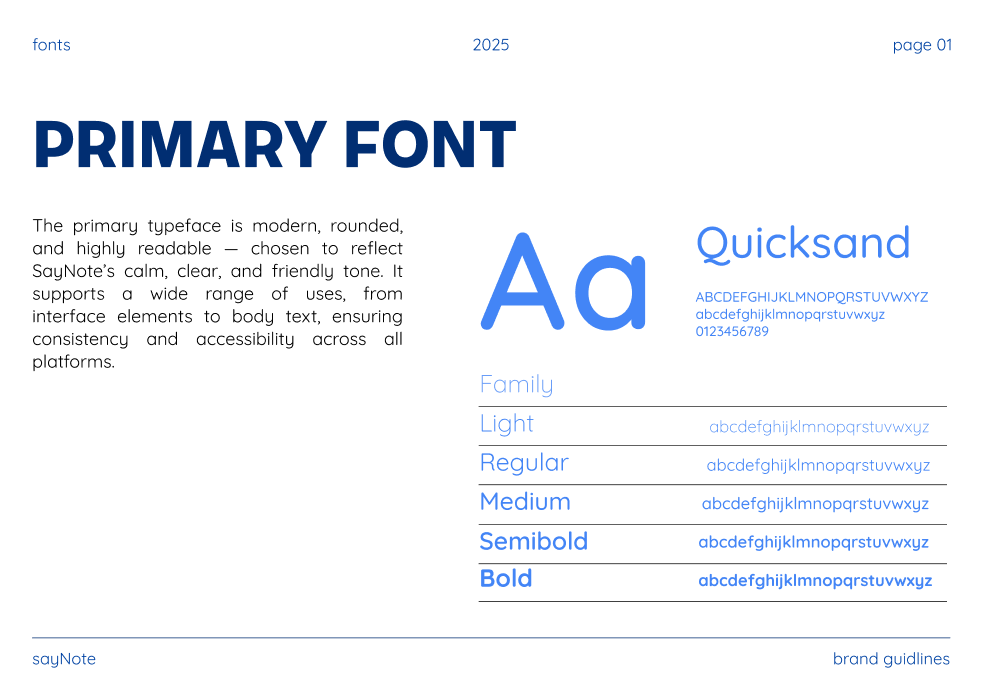
\includegraphics[width=0.7\textwidth]{docs/visual-indentity/pictures/primary-font.png}
    \caption{Police principale SayNote : structure et impact pour les titres. \newline\textit{Cette police renforce la clarté et la hiérarchie visuelle des contenus.}}
\end{figure}
% Explication brève avant chaque figure
\noindent
\textit{La figure suivante illustre un élément clé de l'identité visuelle ou de la communication de la marque.}
\begin{figure}[H]
    \centering
    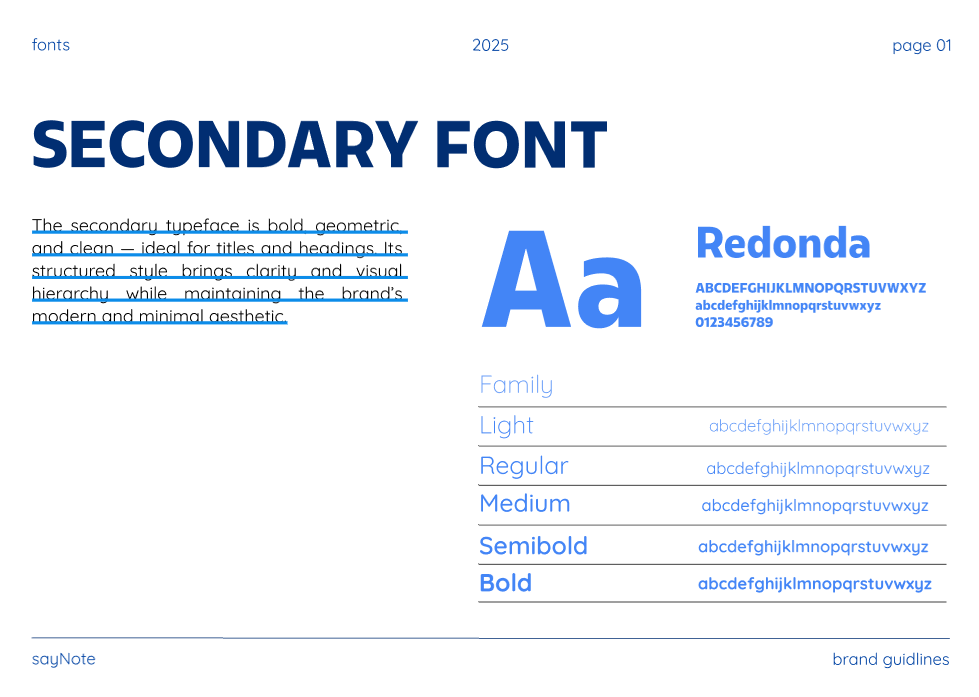
\includegraphics[width=0.7\textwidth]{docs/visual-indentity/pictures/secondery-font.png}
    \caption{Police de contenu SayNote : lisibilité, chaleur et modernité. \newline\textit{Ce choix garantit une lecture agréable et une identité chaleureuse.}}
\end{figure}

\textbf{Titres~:}
Police sans-serif, géométrique, épaisse, pour la clarté et la structure.

\textbf{Corps de texte~:}
Police sans-serif, arrondie et chaleureuse, pour la lisibilité et l’accessibilité.

L’association des deux polices crée un équilibre entre structure et douceur, fidèle à l’esprit VoiceNotion.

\section{Palette de couleurs}
\subsection{Bleu principal — \#4385F6}
Ce bleu vibrant représente la clarté, la confiance et un design intelligent. Il évoque le calme du ciel et la fiabilité des outils numériques modernes. Élément central de l’identité SayNote, il symbolise la concentration, la productivité et la confiance, en parfaite adéquation avec notre objectif d’une expérience vocale sans distraction.

\subsection{Bleus profonds — \#1E6DE0, \#0043A5, \#002E72}
Ces nuances plus sombres complètent la couleur principale en ajoutant profondeur et contraste. Elles reflètent la structure et la clarté de l’interface SayNote, renforçant la stabilité, la précision et une sensation de contrôle calme.

\subsection{Accent clair — \#CFE3FF}
Cet accent pastel doux apporte une touche de légèreté et de joie à l’ensemble de la marque. Il confère une qualité rafraîchissante et aérée à l’interface tout en améliorant la hiérarchie visuelle et l’accessibilité. Il soutient notre ton de clarté et de sérénité, équilibrant les bleus plus soutenus.

% Explication brève avant chaque figure
\noindent
\textit{La figure suivante illustre un élément clé de l'identité visuelle ou de la communication de la marque.}
\begin{figure}[H]
    \centering
    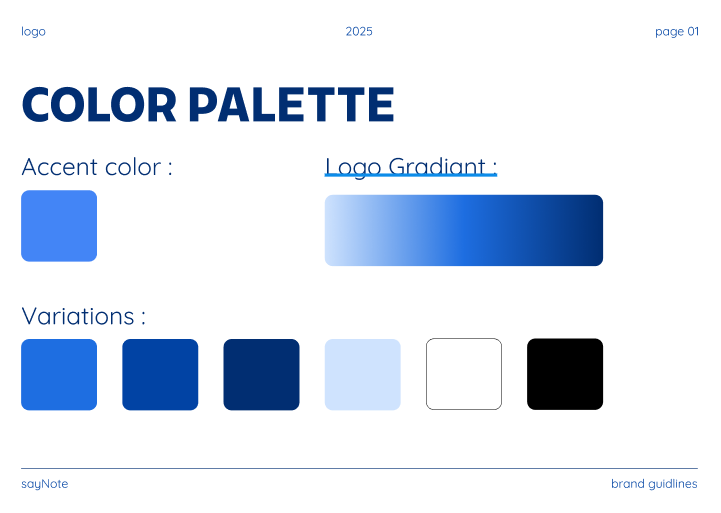
\includegraphics[width=0.6\textwidth]{docs/visual-indentity/pictures/color-palette.png}
    \caption{Palette de couleurs SayNote : harmonie, clarté et confiance.}
\end{figure}

En combinant ces couleurs, SayNote propose un système visuel harmonieux et émotionnellement aligné, reflétant nos valeurs fondamentales : clarté, confiance, inclusivité et productivité sereine.

\section{Stationery \& Visual Imagination}
\subsection{Design}
La papeterie VoiceNotion comprend une gamme complète de supports imprimés, conçus pour refléter l'identité visuelle de la marque et renforcer la cohérence graphique dans toutes les communications professionnelles.

\subsubsection*{Carte de visite}
La carte de visite VoiceNotion reprend les codes graphiques de la marque : couleurs, typographie et logo. Elle offre une présentation professionnelle et mémorable lors des échanges.
% Explication brève avant chaque figure
\noindent
\textit{La figure suivante illustre un élément clé de l'identité visuelle ou de la communication de la marque.}
\begin{figure}[H]
    \centering
    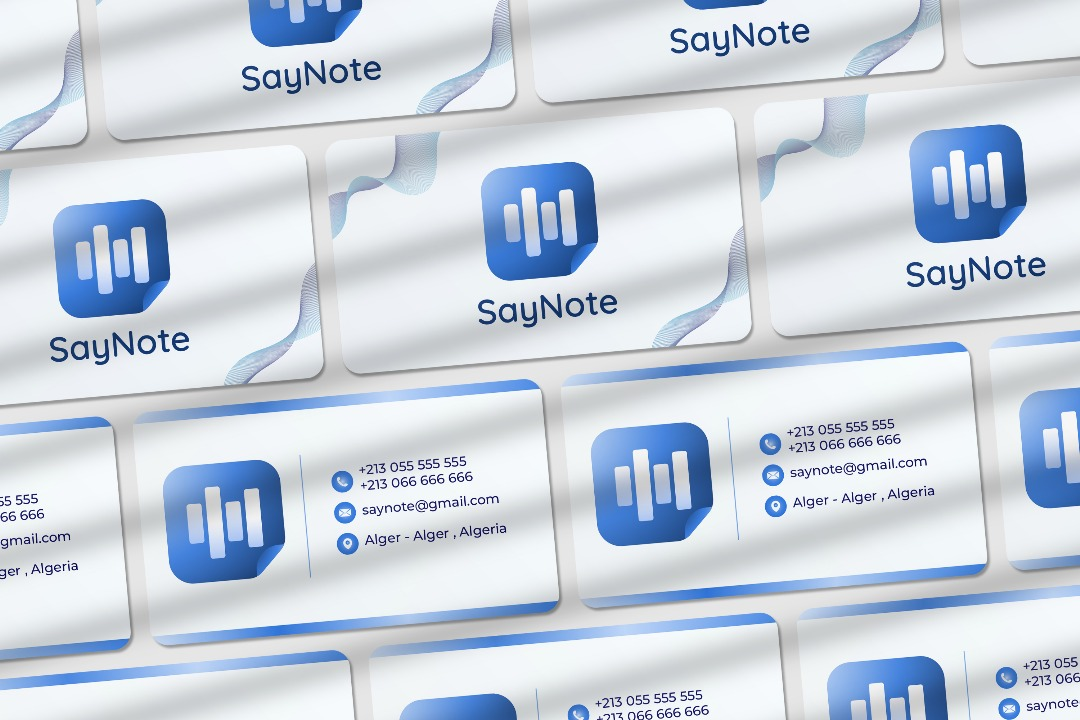
\includegraphics[width=0.5\textwidth]{docs/visual-indentity/pictures/card.jpg}
    \caption{Carte de visite VoiceNotion : design épuré et impactant. \newline\textit{Un support professionnel qui véhicule l'identité de la marque.}}
\end{figure}

\subsection{Poster}
\subsubsection*{a) Concept du design}
Le concept du poster repose sur l'attraction visuelle, l'expression de l'identité de la marque et la mise en avant des fonctionnalités clés de SayNote. La composition soigneusement pensée allie des images frappantes, des couleurs vibrantes de la marque et un texte concis et percutant pour assurer lisibilité et impact. Les posters finaux sont conçus au format A3.

\subsubsection*{b) Versions}
Deux versions de posters ont été réalisées pour répondre à différents usages et publics. La première met l’accent sur la productivité vocale de SayNote, tandis que la seconde valorise la clarté et la fluidité apportées par l’IA et le design. Les deux affiches conservent une cohérence visuelle tout en ciblant des besoins et contextes variés.

\subsubsection*{c) Développement du contenu}
Le contenu a été élaboré pour délivrer un message convaincant : titres accrocheurs, valeurs essentielles et un appel à l’action clair (téléchargement de l’application ou visite du site). Les visuels et le texte reflètent le ton de la marque : calme, clarté, soutien et modernité.

% Explication brève avant chaque figure
\noindent
\textit{La figure suivante illustre un élément clé de l'identité visuelle ou de la communication de la marque.}
\begin{figure}[H]
    \centering
    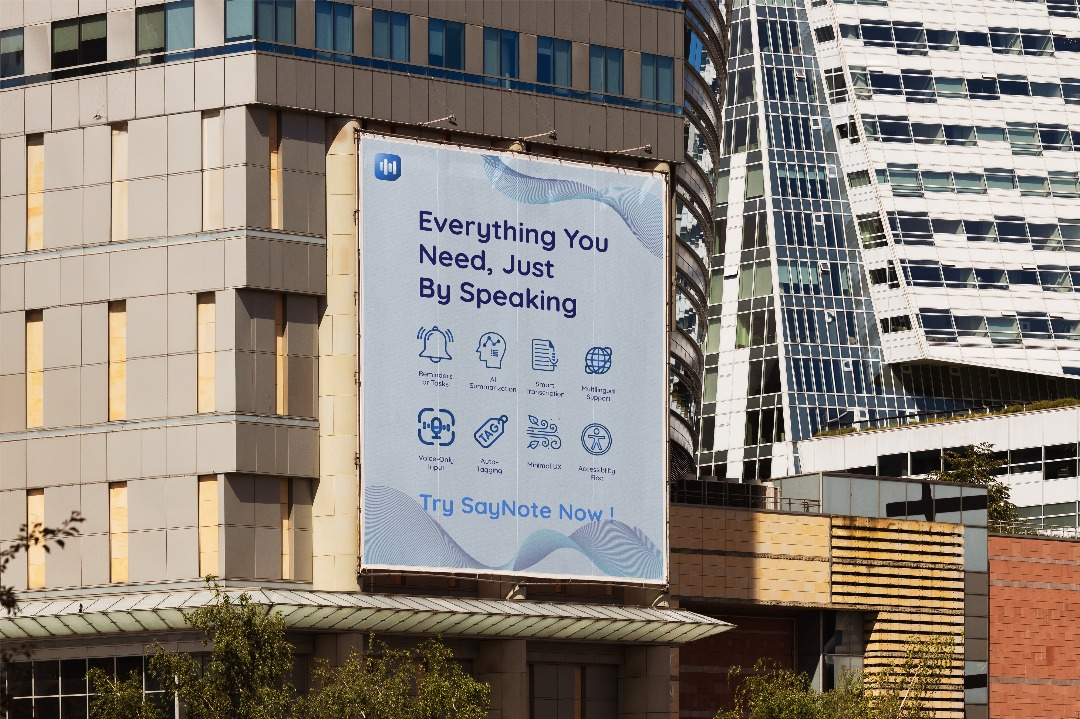
\includegraphics[width=0.8\textwidth]{docs/visual-indentity/pictures/poster2.jpg}
    \caption{Poster VoiceNotion : version "Productivité Vocale" – met en avant la rapidité et la simplicité de la prise de notes par la voix. \newline\textit{Ce poster valorise l'usage vocal et la modernité de l'application.}}
\end{figure}
% Explication brève avant chaque figure
\noindent
\textit{La figure suivante illustre un élément clé de l'identité visuelle ou de la communication de la marque.}
\begin{figure}[H]
    \centering
    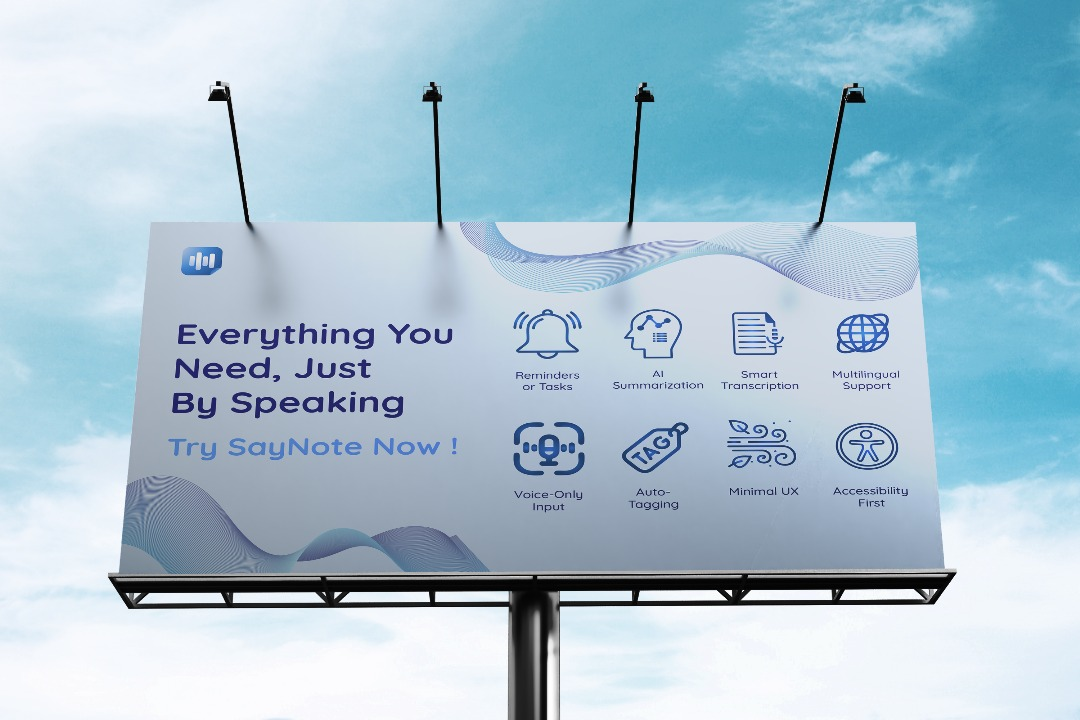
\includegraphics[width=0.8\textwidth]{docs/visual-indentity/pictures/poster.jpg}
    \caption{Poster VoiceNotion : version "Clarté et Innovation" – valorise la fluidité, la technologie et le design moderne de l’application.}
\end{figure}

\subsection{Banner}
\subsubsection*{a) Concept du design}
La bannière VoiceNotion est conçue pour renforcer la présence visuelle de la marque lors d’événements ou dans des espaces digitaux. Elle s’appuie sur une composition graphique forte, des couleurs distinctives et des éléments identitaires pour attirer l’attention et transmettre les valeurs du projet.

\subsubsection*{b) Développement du contenu}
Les messages mis en avant sur la bannière sont pensés pour promouvoir la crédibilité, la modernité et la cohérence de la marque, tout en assurant une lisibilité optimale à distance. Les éléments graphiques sont harmonisés avec l’ensemble de la papeterie et des supports visuels.

\subsubsection*{c) Éléments visuels}
% Explication brève avant chaque figure
\noindent
\textit{La figure suivante illustre un élément clé de l'identité visuelle ou de la communication de la marque.}
\begin{figure}[H]
    \centering
    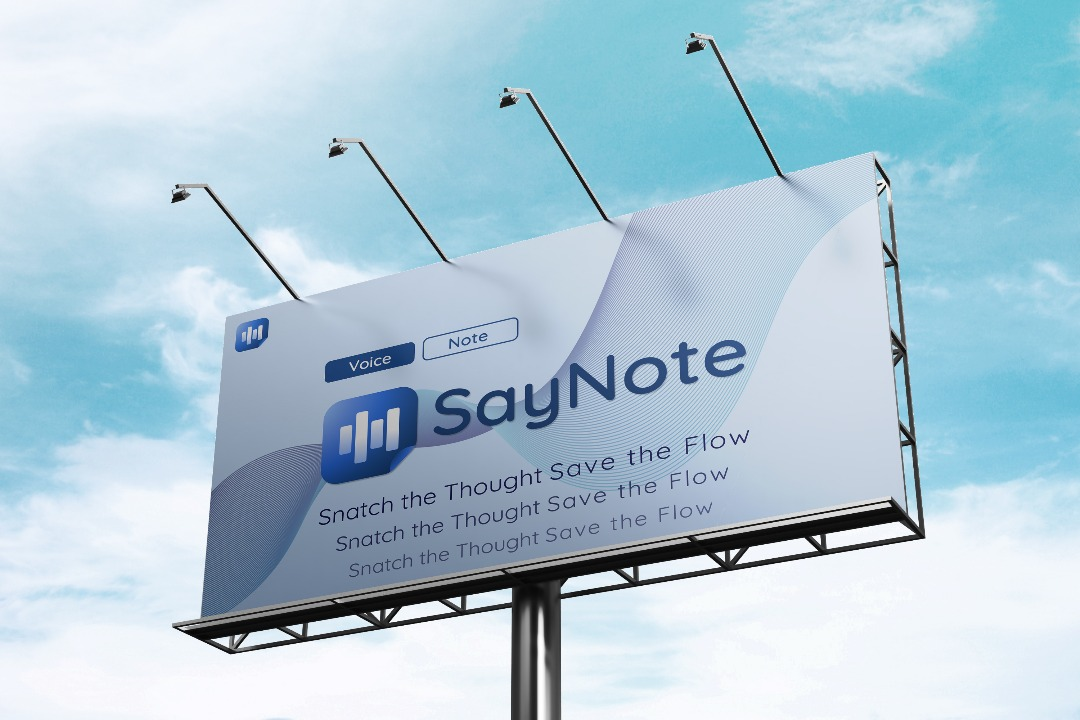
\includegraphics[width=0.8\textwidth]{docs/visual-indentity/pictures/big-banner.jpg}
    \caption{Bannière principale VoiceNotion : composition graphique forte et identité affirmée. \newline\textit{La bannière incarne la présence visuelle de la marque lors d'événements et en ligne.}}
\end{figure}
% Explication brève avant chaque figure
\noindent
\textit{La figure suivante illustre un élément clé de l'identité visuelle ou de la communication de la marque.}
\begin{figure}[H]
    \centering
    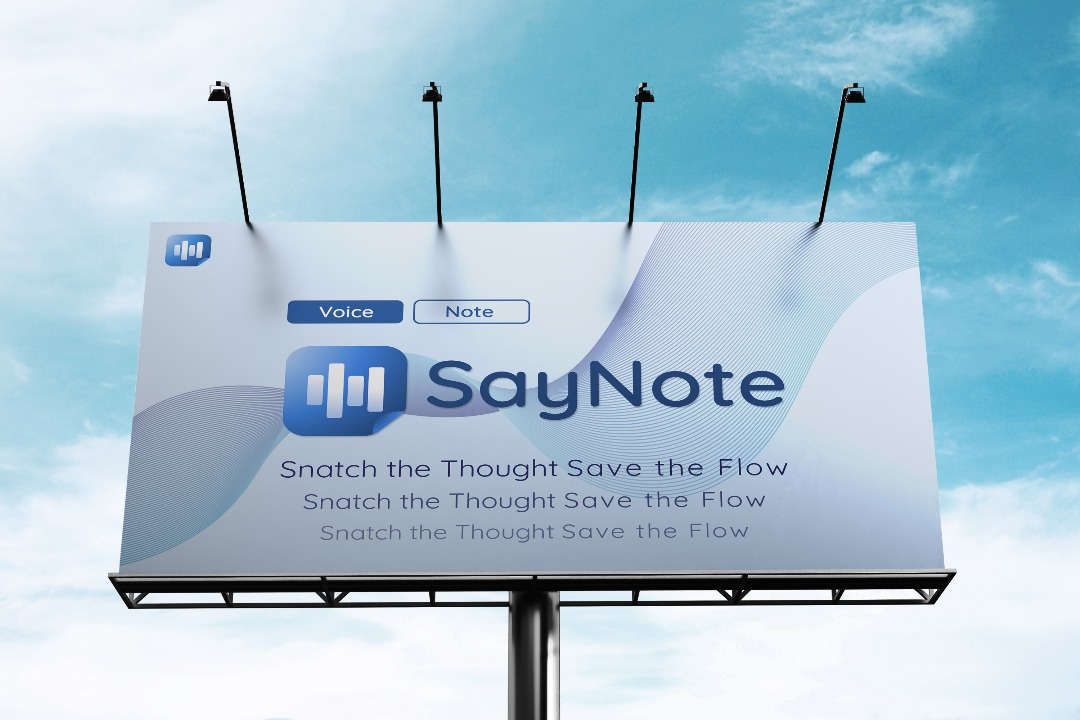
\includegraphics[width=0.8\textwidth]{docs/visual-indentity/pictures/big-banner-directly .jpg}
    \caption{Variante directe de la bannière VoiceNotion : adaptation pour différents contextes visuels. \newline\textit{Cette déclinaison assure la flexibilité de la marque sur divers supports.}}
\end{figure}

\subsection{Flyer (Brochure)}
\subsubsection*{a) Concept du design}
Le flyer VoiceNotion reprend l’ensemble de l’identité visuelle de la marque pour offrir un support de communication synthétique, élégant et professionnel. Il met en avant la cohérence graphique et la qualité des supports imprimés.

\subsubsection*{b) Développement du contenu}
Le contenu du flyer est pensé pour présenter les atouts de la marque et renforcer la reconnaissance auprès du public cible. La sélection d’images illustre la diversité et la qualité des supports :

% Explication brève avant chaque figure
\noindent
\textit{La figure suivante illustre un élément clé de l'identité visuelle ou de la communication de la marque.}
\begin{figure}[H]
    \centering
    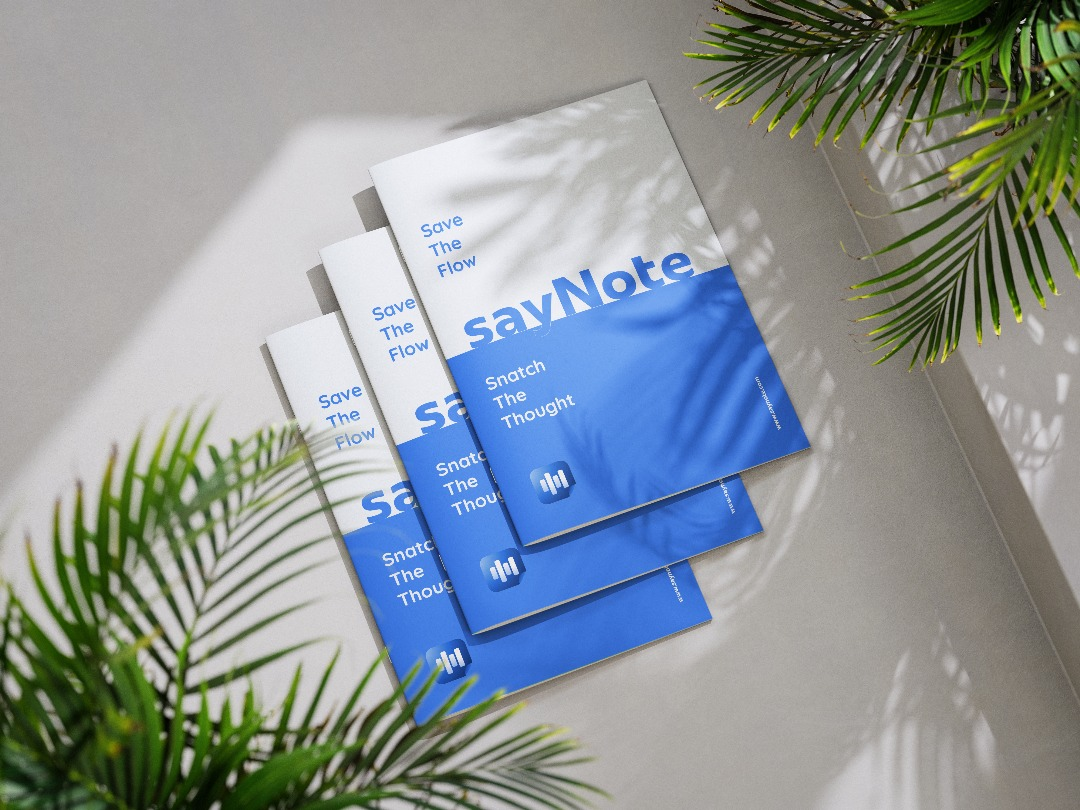
\includegraphics[width=0.7\textwidth]{docs/visual-indentity/pictures/pappiers.jpg}
    \caption{Aperçu général de la papeterie VoiceNotion : enveloppes, blocs-notes et feuilles personnalisées.}
\end{figure}
% Explication brève avant chaque figure
\noindent
\textit{La figure suivante illustre un élément clé de l'identité visuelle ou de la communication de la marque.}
\begin{figure}[H]
    \centering
    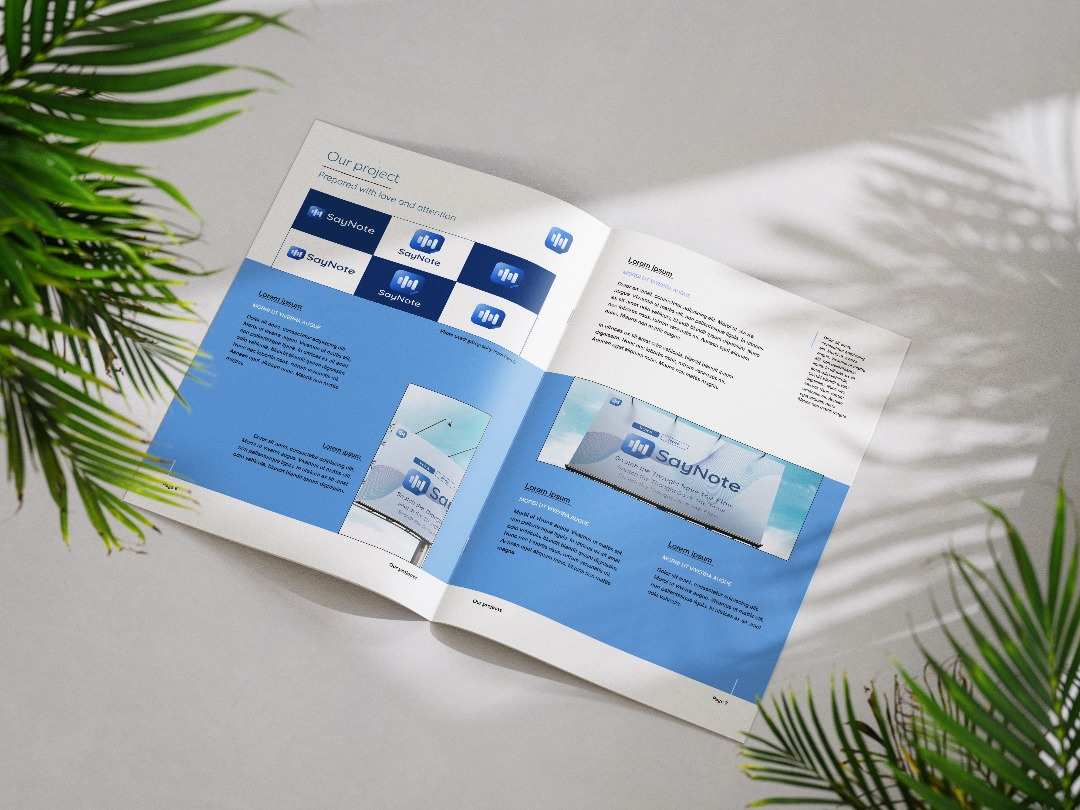
\includegraphics[width=0.7\textwidth]{docs/visual-indentity/pictures/pappier.jpg}
    \caption{Papier à en-tête VoiceNotion : design épuré et professionnel. \newline\textit{Un élément essentiel de la papeterie qui renforce la cohérence de l'identité graphique.}}
\end{figure}
% Explication brève avant chaque figure
\noindent
\textit{La figure suivante illustre un élément clé de l'identité visuelle ou de la communication de la marque.}
\begin{figure}[H]
    \centering
    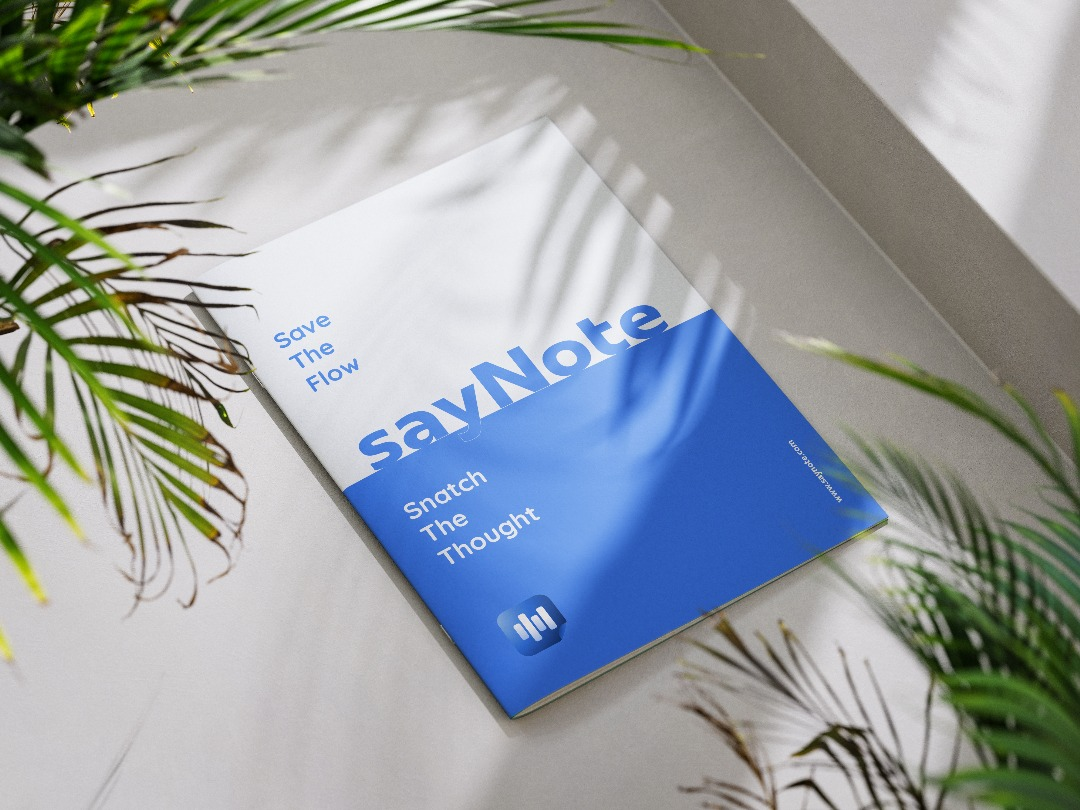
\includegraphics[width=0.7\textwidth]{docs/visual-indentity/pictures/pappier-back.jpg}
    \caption{Verso du papier à en-tête VoiceNotion : souci du détail et harmonie visuelle. \newline\textit{Le verso complète l'expérience de marque jusque dans les moindres détails.}}
\end{figure}


\section{Video Animation}
\subsection{Video scenes}
\subsubsection*{a) Problem presentation}
À compléter.
\subsubsection*{b) Solution presentation}
À compléter.
\subsubsection*{c) Process description}
À compléter.
\subsubsection*{d) Result}
À compléter.

\section{Conclusion}
La création d'une identité de marque est un processus dynamique et itératif qui nécessite une planification minutieuse, de la créativité et une attention aux détails. C'est un voyage continu de perfectionnement et de renforcement de l'identité de la marque afin d'assurer cohérence et pertinence dans un marché en constante évolution. Grâce à un positionnement stratégique, un design visuel, des messages convaincants et une expérience de marque cohérente, les organisations peuvent se différencier de leurs concurrents, établir un lien émotionnel fort avec leur public et favoriser la fidélité à la marque. En investissant du temps et des efforts dans le processus de création de l'identité de marque, les entreprises peuvent poser des bases solides pour un succès à long terme, leur permettant de communiquer efficacement leurs valeurs, de tenir leurs promesses et de laisser une impression durable dans l'esprit des consommateurs. En fin de compte, une identité de marque bien définie devient un atout puissant qui aide les entreprises à prospérer et à avoir un impact significatif dans leurs secteurs respectifs.

% --- Conclusion non numérotée ---
\vspace{1cm}
\begin{center}
\textbf{\large Conclusion du Chapitre}
\end{center}

\noindent
Ce chapitre a mis en lumière l'importance de l'identité visuelle pour VoiceNotion, en détaillant les choix de design, de typographie et de supports graphiques. Une identité forte et cohérente renforce la crédibilité du projet, facilite la reconnaissance de la marque et contribue à offrir une expérience utilisateur mémorable et différenciante. Ces éléments visuels soutiennent la stratégie globale de VoiceNotion et accompagnent son évolution future.
